\chapter{Contesto aziendale}

\section{Azienda ospitante}
% \subsection{Presentazione dell'azienda}
% \begin{figure}[h]
%   \begin{center}
%     
\includegraphics[width=0.20\textwidth]{images/sync_lab_logo.jpg}
%     \caption{Logo dell'azienda ospitante lo \textit{stage}}
%     \captionsetup{aboveskip=1pt}
%     \caption*{\begin{footnotesize}\textit{Fonte:} \url{https://www.synclab.it/}\end{footnotesize}}
%   \end{center}
% \end{figure}
% The \acfoot{ABC}\footnote{this works, too}.
Sync Lab s.r.l.\footfullcite{sync-lab-site} è un'azienda di produzione software, \sacrfoot{ict} e consulenze informatiche nata nel 2002 a Napoli.
L'azienda al suo stato attuale presenta un organico aziendale composto da più di 200 risorse, con un fatturato annuo di 12 milioni, una solida base finanziaria e una diffusione sul territorio a livello nazionale.
Sync Lab possiede delle significative fette di mercato riguardanti lo sviluppo di prodotti nel settore mobile, videosorveglianza e sicurezza delle strutture informatiche aziendali.

L'azienda ha acquisito numerose certificazioni ISO LL-C per attestare la qualità dei servizi forniti.
% \begin{figure}[h]
%   \begin{center}
%     
\includegraphics[width=0.65\textwidth]{images/sync_lab_certifications.png}
%     \caption{Certificazioni ISO LL-C di Sync Lab}
%     \captionsetup{aboveskip=2pt}
%     \caption*{\begin{footnotesize}\textit{Fonte:} \url{https://www.synclab.it/}\end{footnotesize}}
%   \end{center}
% \end{figure}
La certificazione ISO-9001 attesta la gestione della qualità, ISO-14001 la gestione dell'ambiente, ISO-27001 la sicurezza dei sistemi di gestione dati e ISO-45001 la sicurezza nel luogo di lavoro.

Tra i clienti di Sync Lab vi sono ditte a livello nazionale di grandi dimensioni e ampio organico, come Intesa San Paolo, TIM, Vodafone, Enel e Trenitalia che necessitano prodotti di un'elevata sicurezza e adatti al considerevole flusso di dati aziendale.

\begin{figure}[h]
  \begin{center}
    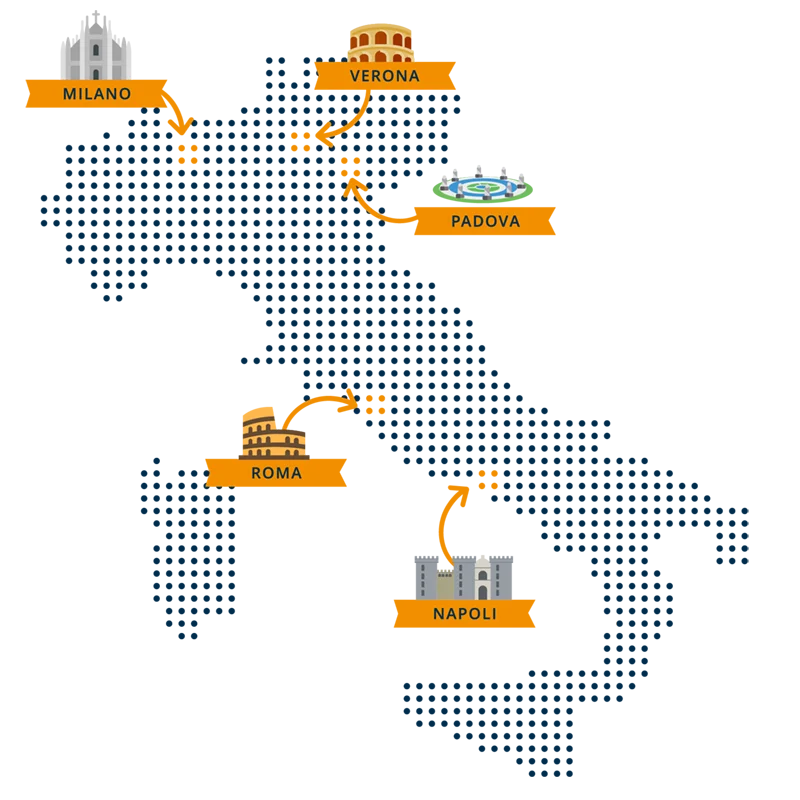
\includegraphics[width=0.45\textwidth]{images/sync_lab_sedi.png}
    \caption{Attuali sedi di Sync Lab}
    \captionsetup{aboveskip=2pt}
    \caption*{\begin{footnotesize}\textit{Fonte:} \url{https://www.synclab.it/}\end{footnotesize}}
  \end{center}
\end{figure}

Sync Lab ha fornito prodotti e consulenze a più di 150 clienti, distribuiti tra clienti diretti e finali, e attualmente possiede cinque sedi (figura \thefigure): Napoli, Roma, Milano, Padova e Verona.

L'azienda è suddivisa in molteplici settori dislocati nelle diverse sedi; l'esperienza personale mi ha portato a conoscere il settore dell'\textit{Enterprise Architecture Integration} e del \textit{Tecnical Professional Services Padova}.

% \bigskip\noindent
% Esposizioni delle ragioni personali che hanno portato alla scelta di tale percorso.


\section{Processi interni e strumenti organizzativi}

% Esposizione delle norme organizzative (\textit{online meeting}, \textit{smart working}, presenze in sede), degli strumenti utilizzati nel rapporto con l’azienda (chat, email e \textit{Project Board}), e delle norme di progetto.
%
% \bigskip\noindent
% Processi interni in cui sono stato coinvolto: Sviluppo, Collaudo, Verifica, Formazione, Manutenzione/Evoluzione.

% \bigskip\noindent
% Breve presentazione dei ruoli delle persone coinvolte nel percorso di \textit{stage}.

L'azienda adotta dei processi interni per delineare l'avanzamento di un progetto.
Sync Lab utilizza una strategia \textit{Agile} per gestire i progetti in modo da consentire un'evoluzione e adattabilità in base alle richieste del cliente e fornire soluzioni \textit{ad-hoc}.

\subsection{Processi interni}

Durante il percorso di \textit{stage} sono stato coinvolto nei processi di Formazione, Progettazione architetturale, Sviluppo, Verifica e Collaudo; i processi di Manutenzione ed Evoluzione sono stati solamente accennati in quanto al di fuori dello scopo del percorso.
Questi processi, nella mia esperienza personale, non sono stati delineati rigorosamente: ciò per garantire libertà e flessibilità allo stagista e all'intero progetto.

\begin{figure}[h]
  \begin{center}
    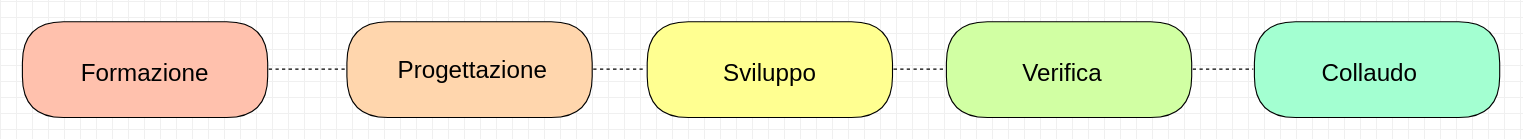
\includegraphics[width=\textwidth]{images/processi.png}
    \caption{Processi interni di cui ho avuto esperienza}
    \captionsetup{aboveskip=2pt}
    \caption*{\begin{footnotesize}\textit{Fonte: elaborazione personale}\end{footnotesize}}
  \end{center}
\end{figure}

Ogni processo è suddiviso in attività modulari, per rendere l'avanzamento efficace e quantificabile (in figura \thefigure\ sono illustrati i processi relativi allo \stage).

Per il processo di Formazione, Sync Lab fornisce materiale sotto forma di corsi \textit{online} tramite le piattaforme \textit{Coursera}\footfullcite{coursera} e \textit{Udemy}\footfullcite{udemy} e diapositive aziendali che illustrano i concetti chiave del settore \sacr{eai}.

Il processo di Sviluppo della mia esperienza personale è risultato abbastanza libero per quanto riguarda le tecnologie e i \software\ utilizzati, purché le scelte fossero adeguatamente motivate e adeguate.

Il processo di Progettazione architetturale è uno dei più complessi, che necessita di una buona dose di esperienza nell'ambito.
Per affrontare questo processo, oltre ad approfondire le mie conoscenze riguardo i diversi \textit{design pattern} e \textit{software architecture style}, l'azienda mi ha accompagnato e supportato nella progettazione stessa, con relative motivazioni.
Il tutor aziendale  Francesco Sanges e il responsabile del settore \sacr{eai} Salvatore Dore
sono stati di fondamentale aiuto in questo processo.

Il processo di Verifica è stato eseguito dal tutor aziendale e dal Responsabile del settore \sacr{eai} a scadenza settimanale, tramite colloqui \textit{online} o resoconti sulla \textit{online board} di riferimento.

Il processo di Collaudo è avvenuto tramite una presentazione \textit{online} e dimostrazione \textit{live} del prodotto sviluppato all'intera azienda.

\subsection{Strumenti organizzativi}

L'organizzazione efficiente di un progetto è garantita dall'utilizzo dei vari strumenti a supporto, quali \textit{Kanban Board} (come \textit{Click Up}\footfullcite{clickup} per la gestione di progetto e \textit{Notion}\footfullcite{notion} per le prenotazioni della postazione di lavoro in sede), \textit{chat} (come \textit{Google Chat}\footfullcite{google-chat}) per i confronti rapidi con gli altri membri interni al progetto ed e-mail per le comunicazioni con componenti esterni al progetto.

Lo strumento più utilizzato in ambito organizzativo durante il mio percorso è la \textit{Kanban Board} di \textit{Click Up}, che ha permesso la gestione, il confronto, la quantificazione e la verifica del progresso.
La figura seguente illustra uno \textit{screenshot} che raffigura lo stato dell'avanzamento.

\bigskip
\begin{figure}[h]
  \begin{center}
    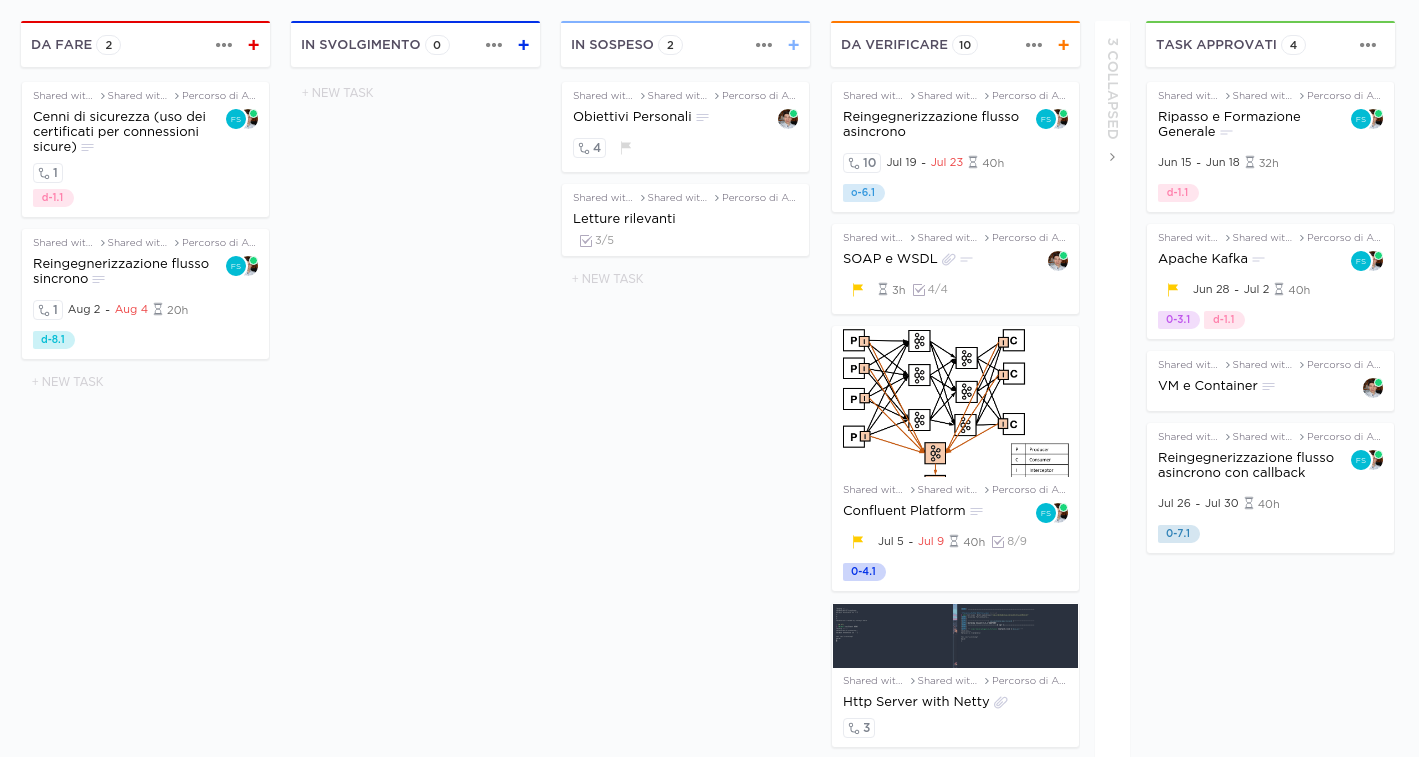
\includegraphics[width=\textwidth]{images/clickup_board_v2.png}
    \caption{\textit{Kanban Board} del progetto di \textit{stage}}
    \captionsetup{aboveskip=2pt}
    \caption*{\begin{footnotesize}\textit{Fonte: elaborazione personale}\end{footnotesize}}
  \end{center}
\end{figure}

Le attività (\textit{task}) vengono inizialmente create nella colonna "DA FARE" dal tutor aziendale o da me, ove ritenuto opportuno.
Per dimostrare l'avanzamento il \textit{task} si sposta verso destra a seconda dello stato raggiunto; lo stagista ha la responsabilità del cambiamento di stato fino alla colonna "DA VERIFICARE", dopodichè è compito del tutor aziendale la verifica e lo spostamento del \textit{task} in "TASK APPROVATI", che comporta l'approvazione finale e conclusione dell'attività.

Per tenere traccia del lavoro svolto riguardante una specifica attività ho utilizzato le \textit{card} messe a disposizione dalla piattaforma, che mi hanno consentito di delineare precisamente la pianificazione e descrizione dell'avanzamento in dettaglio del singolo \textit{task}.

\begin{figure}[H]
  \begin{center}
    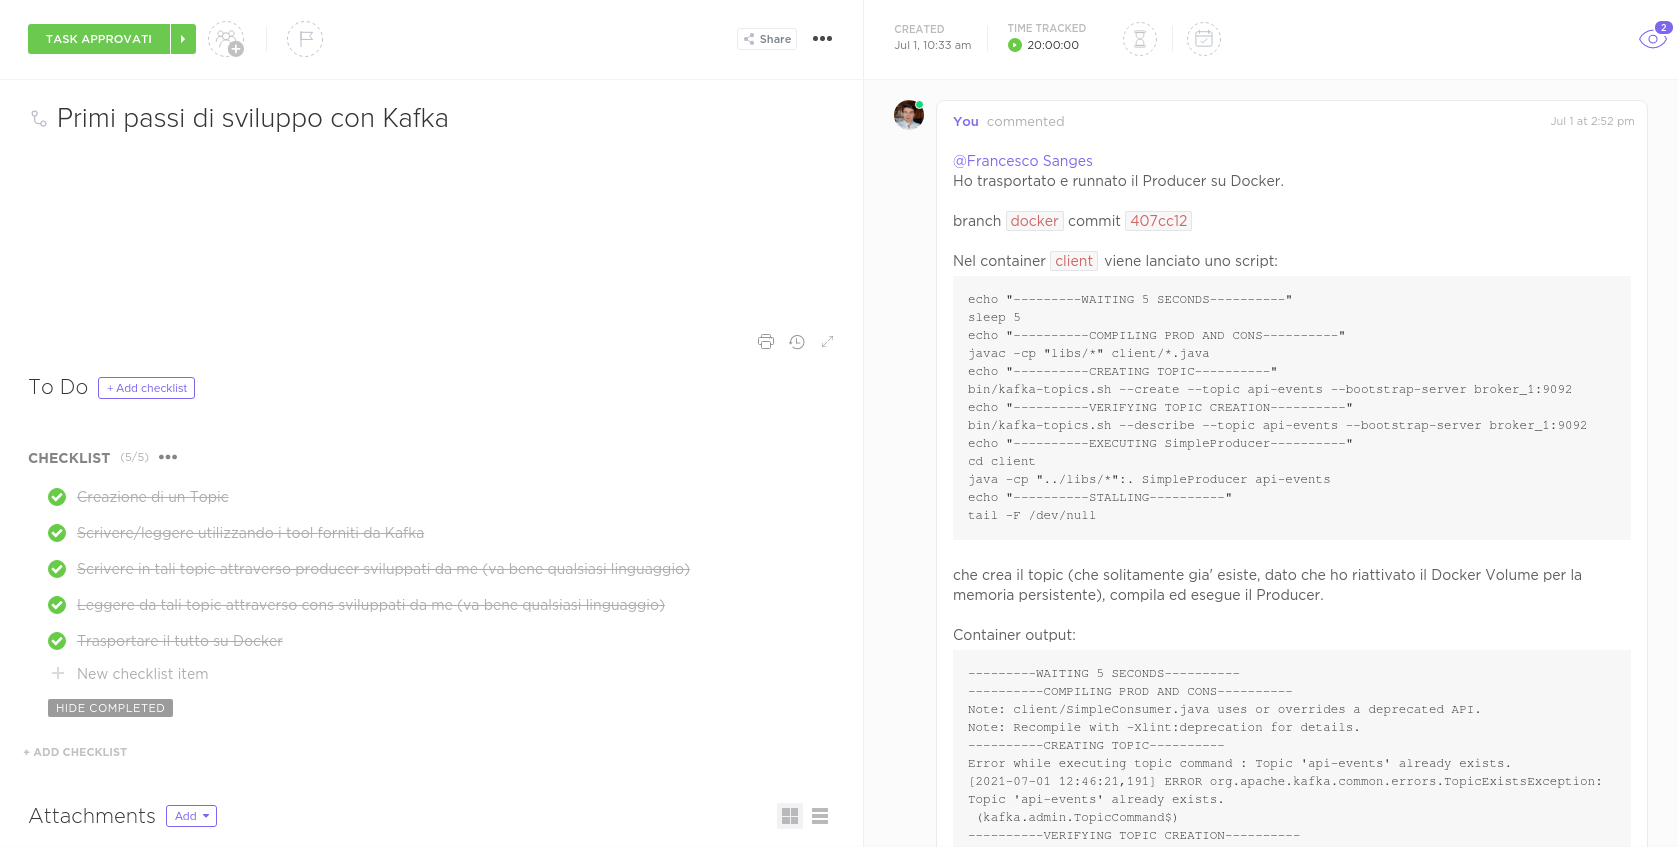
\includegraphics[width=\textwidth]{images/clickup_task_v2.png}
    \caption{Esempio di un'attività del processo di Formazione}
    \captionsetup{aboveskip=2pt}
    \caption*{\begin{footnotesize}\textit{Fonte: elaborazione personale}\end{footnotesize}}
  \end{center}
\end{figure}

Questa \textit{card} contiene una casella di testo per inserire una descrizione e appunti utili ove sia richiesto, una \textit{checklist} approfondita, e una colonna che mantiene uno storico dei commenti; quest'ultima colonna non solo permette a me di mantenere un'importante resoconto sul lavoro svolto, ma consente anche al tutor aziendale e esperti del settore di quantificare il progresso e di fornire un aiuto rapido e contestuale.



\section{Ambiente di lavoro}

% Sviluppo indipendente dal sistema operativo, produzione di \software\ non strettamente legati ad uno specifico linguaggio, utilizzo di ambienti virtuali quali \textit{Virtual Machine} e \textit{container} per simulare sistemi indipendenti.
L'ambiente di lavoro di cui ho avuto esperienza risulta libero e flessibile.
Lo sviluppo del prodotto nell'ambito del \sacr{eai} dev'essere indipendente dal linguaggio di programmazione, dagli strumenti utilizzati per l'esecuzione e sviluppo, e possibilmente anche dal Sistema Operativo su cui eseguire il \software.
A tal scopo si utilizzano strumenti quali \textit{Virtual Machine} e \textit{Container}: essi non solo garantiscono l'indipendenza dal Sistema Operativo in uso, ma simulano efficacemente il caso d'uso reale in cui gli eseguibili sono dislocati in più dispositivi come spesso accade per il cliente finale.
Nonostante il percorso formativo abbia visto l'apprendimento di entrambe le tecnologie tramite l'utilizzo dei \software\ \textit{Virtual Box}\footfullcite{virtualbox} e \textit{Docker}\footfullcite{docker}, solo quest'ultima è stata utilizzata durante il progetto.

Un altro concetto fondamentale che caratterizza l'ambiente di lavoro nel campo del \sacr{eai} è quello del sistema distribuito, di cui l'azienda ha un forte interesse per soffisdare le necessità dei suoi clienti.

\begin{figure}[h]
  \begin{center}
    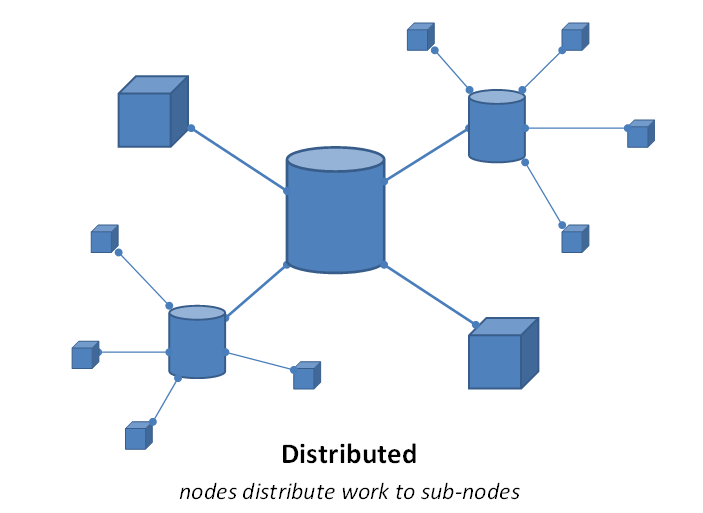
\includegraphics[width=0.45\textwidth]{images/distributed.png}
    \caption{Illustrazione di un sistema distribuito}
    \captionsetup{aboveskip=2pt}
    \caption*{\begin{footnotesize}\textit{Fonte:} \url{https://www.delphitools.info/DWSH/}\end{footnotesize}}
  \end{center}
\end{figure}

Un sistema distribuito (figura \thefigure) è una collezione di componenti indipendenti (spesso collocati in macchine differenti) che condividono dei messaggi fra di loro per raggiungere un obiettivo comune.
Una'architettura software basata su di un sistema distribuito necessita di una rete che connette tutti i singoli componenti (macchine, \textit{hardware} o \textit{software}), cosicchè sia possibile lo scambio dei messaggi.




% \begin{figure}[h]
%   \begin{center}
%     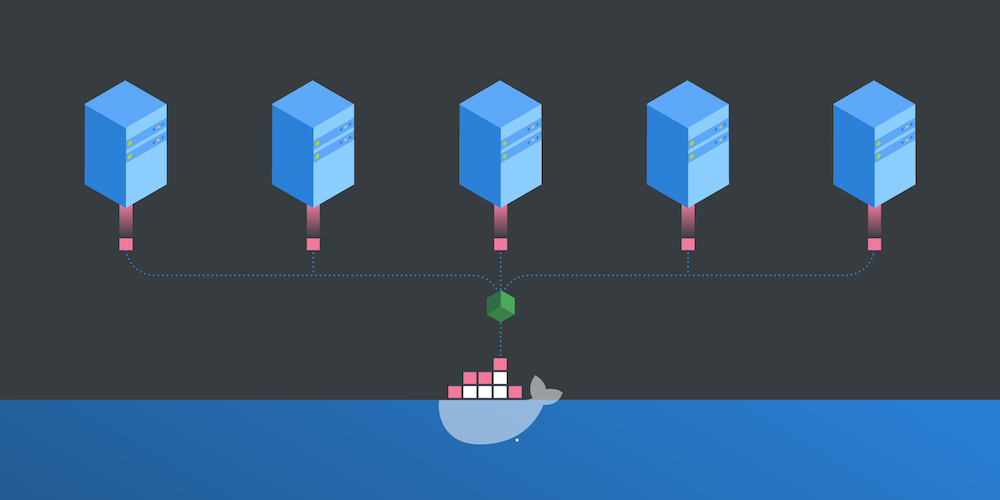
\includegraphics[width=0.75\textwidth]{images/docker_compose.png}
%     \caption{Illustrazione di un sistema a servizi indipendenti in container Docker}
%     \captionsetup{aboveskip=2pt}
%     \caption*{\begin{footnotesize}\textit{Fonte:} \url{https://pspdfkit.com/blog/2018/how-to-use-docker-compose-to-run-multiple-instances-of-a-service-in-development/}\end{footnotesize}}
%   \end{center}
% \end{figure}


\subsection{Servizi offerti dall'azienda}

Per comprendere appropriatamente il contesto che ha portato alla nascita del progetto di \stage\, è bene conoscere la tipologia di servizi e prodotti che l'azienda offre ai propri clienti.
Sync Lab offre per i propri clienti numerosi servizi, tra cui:
\begin{itemize}
  \item Valutazione e controllo progetti
    \begin{itemize}
      \item \textit{Planning e project management}; definizione di \textit{Milestone} e \textit{team} di progetto.
      \item Valutazione di impatto e \textit{risk analysis}; monitoraggio e \textit{benchmarking}.
      \item Valutazione e controllo di progetti \software\ attraverso l’utilizzo di metriche e modelli economici di stima e previsione.
    \end{itemize}
    \item Sistemi distribuiti di \textit{Enterprise}
      \begin{itemize}
        \item Progettazione e realizzazione di sistemi distribuiti \textit{Enterprise} in architettura \sacrfoot{j2ee}, \sacrfoot{ejb}, \sacrfoot{cobra} e \textit{Web Services}.
        \item Progettazione e realizzazione di sistemi basati su \sacrfoot{mom} e \sacrfoot{jms}.
      \end{itemize}
    \item Tecnologie \textit{\acrlong{oo}}
    \begin{itemize}
      \item Applicazione delle tecnologie \sacr{oo} all’analisi e progettazione di \software\ applicativo e di sistema e nella definizione di architetture distribuite \textit{enterprise}.
      \item Utilizzo di metodologie \sacr{oo} per progettazione di applicazioni e processi e \sacr{uml}, con supporto di strumenti di \textit{modeling}, applicazione e definizione di \textit{Design Pattern}.
    \end{itemize}
\end{itemize}

\section{Dominio applicativo}

\subsection{\sacr{eai} e \textit{Middleware}}

% L'esperienza di \textit{stage}
% Breve introduzione al settore del \textit{Enterprise Application Integration}, al tipo di clientela (ovvero pubblica e privata di grandi dimensioni, big data), alla tipologia di \software\ prodotti dall’azienda per la clientela (\textit{Middleware}), e alla propensione all’innovazione (richieste da parte della clientela
% In conclusione al percorso di studi del corso di laurea in Informatica ho effettuato lo \textit{stage} presso \textit{Sync Lab}.
% Sync Lab è un'azienda di produzione \software\ e integrazione di sistemi che fornisce principalmente prodotti a clienti di grande dimensione, sia pubblici che privati.
\begin{figure}[h]
  \begin{center}
    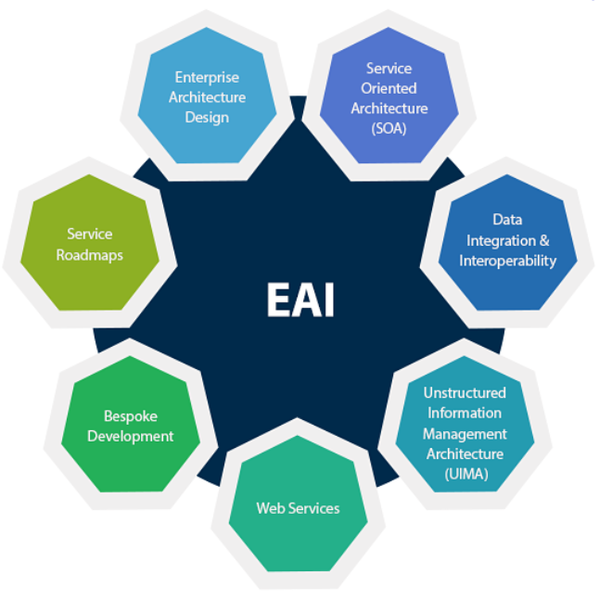
\includegraphics[width=0.65\textwidth]{images/eai.png}
    \caption{Concetti principali del \sacr{eai}}
    \captionsetup{aboveskip=2pt}
    \caption*{\begin{footnotesize}\textit{Fonte:} \url{https://commons.wikimedia.org/wiki/File:KrisangelChap2-EAI.png}\end{footnotesize}}
  \end{center}
\end{figure}

Il percorso di \textit{stage} intrapreso è associato al settore del \textit{Enterprise Architecture Integration}, che si occupa principalmente del \sacr{eai} (\textit{\acrlong{eai}}, figura \thefigure) ovvero dell'integrazione funzionale di applicazioni aziendali per una clientela di grandi dimensioni (come un'azienda di telecomunicazioni), tramite sistemi di integrazione e \textit{Middleware}.

I \textit{Middleware} e sistemi di integrazione prodotti comprendono l'utilizzo di molteplici linguaggi e tecnologie in continua evoluzione.\\
Dal sito di Red Hat\footfullcite{red-hat-middleware}:
% Dal sito di Red Hat\footnote{\textit{Cos'è il Middleware?}\url{https://www.redhat.com/it/topics/middleware/what-is-middleware}}:
\begin{displayquote}
  \textit{Il middleware è un software che fornisce alle applicazioni servizi e capacità frequentemente utilizzati, tra cui gestione dei dati e delle API, servizi per le applicazioni, messaggistica e autenticazione.\\
  Aiuta gli sviluppatori a creare le applicazioni in modo più efficiente e agisce come un tessuto connettivo tra applicazioni, dati e utenti.\\
  Può rendere conveniente lo sviluppo, l'esecuzione e la scalabilità di applicazioni alle organizzazioni con ambienti multicloud e containerizzati.}
\end{displayquote}
\noindent
I \textit{Middleware} pertanto vedono due importanti utilizzi nel settore \sacr{eai}:
\begin{itemize}
  \item \textbf{Integrazione su più livelli:} i \textit{Middleware} connettono i principali sistemi aziendali interni ed esterni. Capacità di integrazione quali trasformazione, connettività, componibilità e messaggistica enterprise, abbinate all'autenticazione \sacrfoot{sso}, aiutano gli sviluppatori a estendere tali capacità su diverse applicazioni.
  \item \textbf{Flussi di dati:} le \sacrfoot{api} rappresentano una modalità per condividere i dati tra le applicazioni. Un altro approccio è quello del flusso di dati asincrono, che consiste nella replica di un set di dati in un livello intermedio, da cui i dati possono essere condivisi con più applicazioni.
  \item \textbf{Ottimizzazione di applicazioni esistenti:} con l'adozione del \textit{Middleware}, gli sviluppatori possono trasformare le applicazioni monolitiche esistenti in applicazioni \textit{cloud native} o a microservizi, mantenendo i validi strumenti già in uso ma migliorandone prestazioni e portabilità (figura \thefigure).
\end{itemize}

\begin{figure}[h]
  \begin{center}
    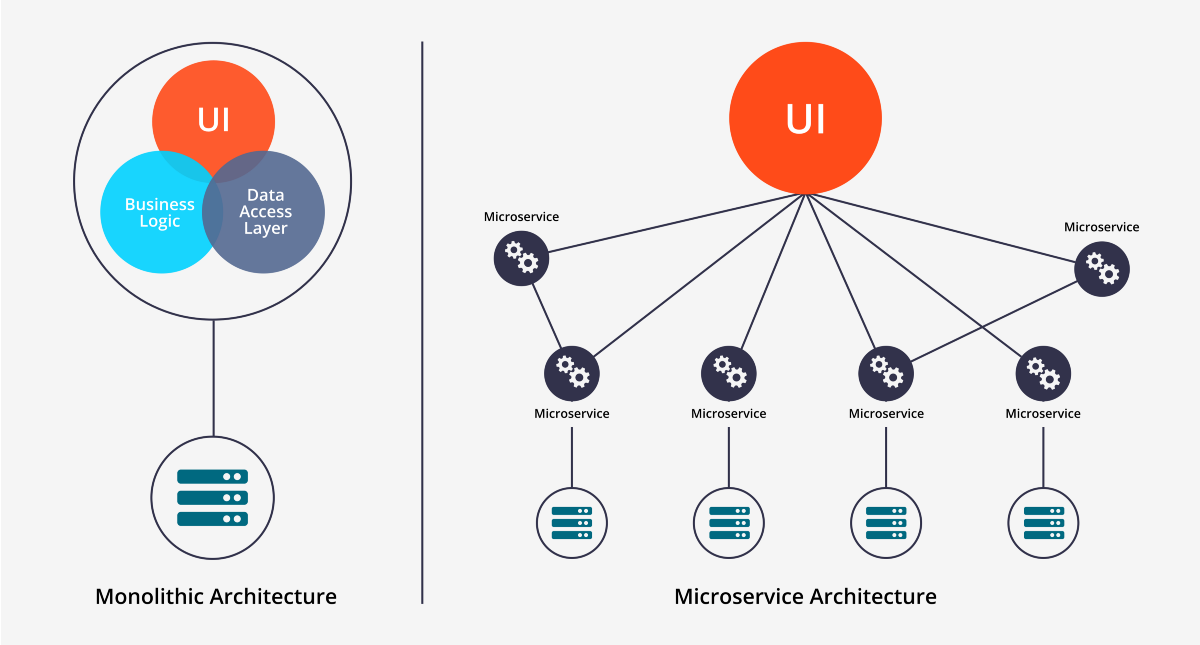
\includegraphics[width=0.85\textwidth]{images/mono_to_micro.png}
    \caption{Dalle classiche soluzioni monolitiche ai moderni sistemi a microservizi}
    \captionsetup{aboveskip=2pt}
    \caption*{\begin{footnotesize}\textit{Fonte:} \url{https://aymax.fr/en/why-a-microservices-architecture/}\end{footnotesize}}
  \end{center}
\end{figure}


\subsection{\textit{Container} e \textit{Virtual Machine}}

Come anticipato nella sezione precedente, tra le tecnologie più utilizzate in questo settore aziendale vi sono molte piattaforme che permettono di simulare ambienti distribuiti su più macchine fisiche, ove possibile anche indipendenti dal Sistema Operativo su cui viene eseguito il prodotto software.

La simulazione di questi \textit{distributed environment} avviene grazie a sistemi basati sul concetto di \textit{container} (come Docker e Kubernetes) oppure interi Sistemi Operativi che vengono eseguiti all'interno di una \textit{Virtual Machine}.
Il vantaggio principale di queste tecnologie è che rendono l'esecuzione del software al loro interno completamente indipendente dall'ambiente circostante, eliminando problemi di \sacrfoot{os} differenti tra i componenti del team o tra l'azienda e i clienti o divergenze nelle dipendenze con relative versioni.
Un \textit{container} o una \textit{Virtual Machine} contengono tutto il necessario affinchè sia possibile eseguire il software al suo interno su diverse macchine fisiche (o anch'esse  virtuali).

Queste piattaforme non solo rendono agevole l'esecuzione del software prodotto, ma anche lo sviluppo: la condivisione, \textit{debugging} e manutenzione risultano più agevoli grazie alla condivisione dell'intero \textit{container} o \sacr{vm} con gli altri membri del team.

Inoltre, si adattano particolarmente bene a simulare l'ambiente distribuito, un concetto fondamentale nel settore del \textit{eai}; infatti è sufficiente generare molteplici \textit{container} o \sacr{vm} sulla stessa macchina fisica per simulare un sistema composto da più macchine fisiche distinte, minimizzando l'utilizzo di risorse senza compromettere il risultato del prodotto finale.
È così possibile per l'azienda riprodurre un sistema complesso che si avvicina alle risorse ed esigenze effettive del cliente, che usualmente possiede molti computer e server dislocati.

\begin{figure}[h]
  \begin{center}
    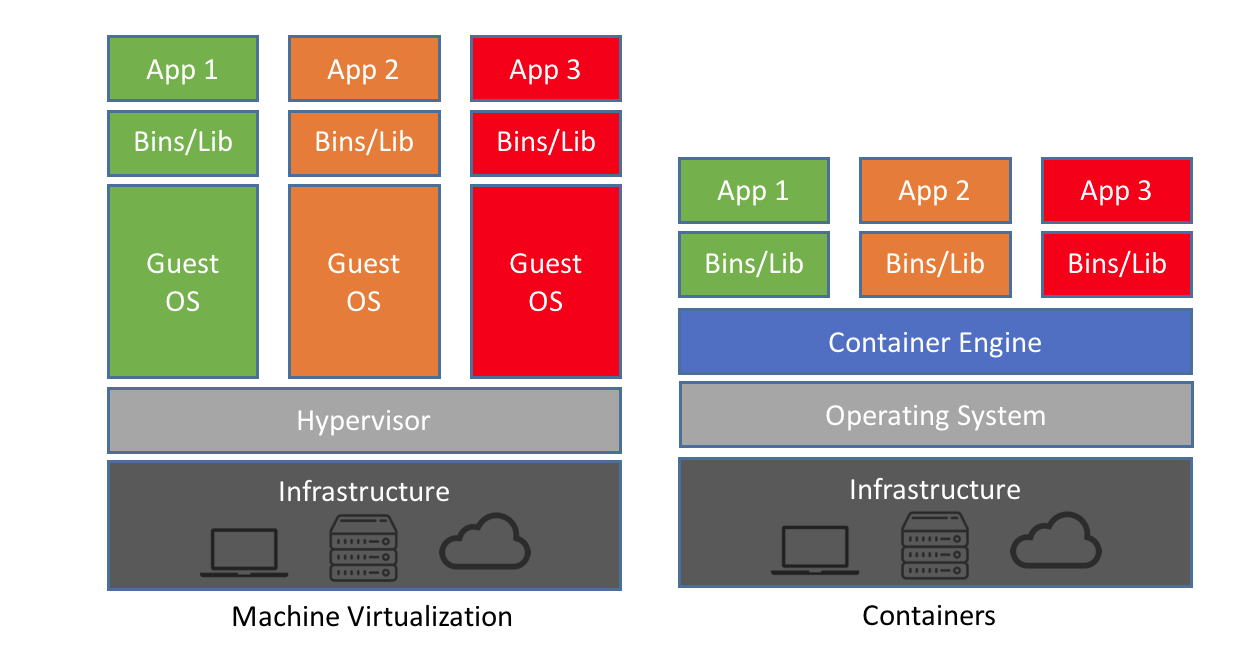
\includegraphics[width=0.85\textwidth]{images/vm_vs_container.png}
    \caption{Differenti implementazioni legate alle \sacr{vm} e \container}
    \captionsetup{aboveskip=2pt}
    \caption*{\begin{footnotesize}\textit{Fonte:} \url{https://pawseysc.github.io/container-workflows/01-docker-intro/index.html}\end{footnotesize}}
  \end{center}
\end{figure}

La figura \thefigure\ rappresenta graficamente le due diverse implementazioni delle due tecnologie.
Vi sono dunque delle notevoli differenze, vantaggi e svantaggi tra l'utilizzo dell'una e dell'altra, tra cui:
\begin{enumerate}
  \item i \container\ sono più rapidi delle \sacr{vm} nell'esecuzione;
  \item i \container\ sono più leggeri delle \sacr{vm} in termini di memoria;
  \item i \container\ sono più adatti a simulare un'architettura a microservizi, dato la relativa semplicità ed efficienza rispetto ad una \sacr{vm};
  \item le \sacr{vm} sono considerate tendenzialmente più sicure dei \container\;
  \item le infrastrutture e strumenti di gestione di grandi quantità di \sacr{vm} sono più consolidate dei corrispettivi strumenti associati ai \container.
\end{enumerate}

% Dati questi presupposti, ho optato per l'implementazione di un sistema basato su i \container\ nel mio progetto di \stage.
Durante il percorso di stage ho approfondito le mie conoscenze riguardo entrambe le tecnologie, optando di utilizzare i \container\ all'interno del mio progetto di \stage, poichè più efficiente considerate le risorse a mia disposizione.
La scelta della piattaforma di \container\ è stata quella di Docker.
% La scelta, in accordo con il tutor aziendale, è dovuta
Più precisamente, ho utilizzato l'estensione \textit{Docker-compose}\footfullcite{docker-compose} per gestire in modo elegante la generazione e collaudo di più servizi indipententi (figura \thefigure): non solo questo \software\ consente di creare velocemente una rete di \textit{container} comunicanti su di una rete isolata, ma rende anche rapido ed efficiente lo sviluppo grazie alla possibilità di modificare e riavviare rapidamente un singolo servizio.
Il caso d'uso realizzato nel mio percorso ha simulato grazie ai \container\ un sistema a microservizi che simula le risorse di un grande cliente gestore di telecomunicazioni, secondo una visione coerente con il tipo di clientela reale dell'azienda.

% TODO: completare il collegamento tra sopra e sotto;
% TODO: magari ci sta bene un esempio di dockerfile

Questo contesto dell'integrazione aziendale porta dunque l'impresa ad avere un'importante propensione all'innovazione, talvolta esplicitamente richiesta dai clienti.
Una direzione dell'evoluzione attuale nel settore \sacr{eai} riguarda la migrazione verso sistemi sempre più distribuiti, in grado di gestire efficacemente ed in tempo reale flussi di dati in continua crescita.
L'avanguardia tecnologica è uno dei principali temi dell'azienda, che garantisce che essa rimanga sempre competitiva sul mercato dei sistemi di integrazione (nel settore dell'\sacr{eai}).
